% Definitions: research/METHODS.md, research/METRICS.md; src/sparsity_research/ceilings.py.
% Training settings: Analysis018 tables/training-protocol.md; Runs004/018/019/032/034 configs and manifests.
% Cohorts/evaluation: Analysis024 data/paper-checkpoints.json; Analysis018 figure_data.json.
% Baseline trajectories: Analysis021 observations/O007-a0-optimization.md;
% relabeled without changing data in Analysis024 observations/040-experimental-setup.md.
\section{Experimental setup details}
\label{app:experiment}

\subsection{Pythia architecture and intervention sites}
\label{app:sites}

Table~\ref{tab:sites} gives the shapes and positions of the sites in
Figure~\ref{fig:pythia-block}. Here $T$ is sequence length, $d$ hidden width,
$d_f$ FFN width and $H$ the number of heads, each with dimension $d_h=d/H$.
Sites and threshold are shared across layers.

\begin{table}[ht]
\centering\small
\caption{Activation shapes and intervention positions for one sequence.}
\label{tab:sites}
\vspace{4pt}
\begin{tabularx}{\linewidth}{@{}lllX@{}}
\toprule
Site & Shape & Following matrix product & Position \\
\midrule
$a$ & $T\!\times\!d$ & QKV projection & After attention LayerNorm \\
$m$ & $T\!\times\!d$ & FFN up projection & After FFN LayerNorm \\
$h$ & $T\!\times\!d_f$ & FFN down projection & Activation-function output \\
$q,k$ & $H\!\times\!T\!\times\!d_h$ & Attention scores & After RoPE \\
$v$ & $H\!\times\!T\!\times\!d_h$ & Probability--value & After the QKV split \\
$z$ & $T\!\times\!d$ & Attention-output projection & Concatenated attention context \\
\bottomrule
\end{tabularx}
\end{table}

\FloatBarrier
\subsection{Architecture-specific sparsity ceilings}
\label{app:architecture-counts}

For one sequence, each Pythia block uses $3Td^2$ scalar multiplications
in the QKV projection, $Td^2$ in the attention-output projection,
$Td d_f$ in each FFN projection, and $dT(T+1)/2$ in each of $QK$ and $PV$.
With $L$ layers and vocabulary size $V_{\mathrm{vocab}}$, the totals are
\begin{equation}
\begin{split}
C_{\mathrm{block}}&=T(4d^2+2dd_f)+dT(T+1),\\
C_{\mathrm{model}}&=LC_{\mathrm{block}}+TdV_{\mathrm{vocab}}.
\end{split}
\label{eq:denominator}
\end{equation}
Sequence count cancels from the ceiling ratio. For $d_f=4d$, per-layer counts
in the ceiling numerator are $0$ for $T_0/P_0$, $4Td^2$ for $T_1/P_0$ and
$T_1/P_1$, $12Td^2$ for $T_4$, and $C_{\mathrm{block}}$ for $T_7$.
For $T_2$, the per-layer numerator is $Tdd_f+Td^2$, covering the FFN-down and attention-output projections; with $d_f=4d$, this becomes $5Td^2$.
Multiplying by $L/C_{\mathrm{model}}$ gives $\Smax$, independent of pressure placement.

Table~\ref{tab:interventions} uses $V_{\mathrm{vocab}}=50{,}304$ and
% Scale extension: analyses/038-2026-09-24-base-t2-t7-scale-frontier/observations/003-manuscript-integration.md; 04_manuscript_evidence.py.
$(L,d)=(6,128),(6,256),(6,512),(24,1{,}024)$ for 14M, 31M, 70M and 410M, respectively,
with the common sequence length in Table~\ref{tab:training-settings}.%
\footnote{Pinned architecture configurations:
\href{https://huggingface.co/EleutherAI/pythia-14m-deduped/blob/7386d9a4ae45aef494a6e704910394def3037fc5/config.json}{14M},
\href{https://huggingface.co/EleutherAI/pythia-31m-deduped/blob/b7782556ba7adfb4730d9bda7d12aa44d88fa132/config.json}{31M},
\href{https://huggingface.co/EleutherAI/pythia-70m-deduped/blob/e93a9faa9c77e5d09219f6c868bfc7a1bd65593c/config.json}{70M}, and
\href{https://huggingface.co/EleutherAI/pythia-410m-deduped/blob/b5e8535141902c0e985cea61fd02afe7fe86af32/config.json}{410M}.}

The 31M configuration has six layers, hidden width 256, FFN width 1,024, eight heads of dimension 32, vocabulary size 50,304 and 30,494,720 trainable parameters.

\begin{table}[!htbp]
\centering\small
\caption{\textbf{Training settings across model sizes.}
Effective batch size equals microbatch size times gradient accumulation.
The common training budget gives fewer tokens per parameter at larger sizes.}
\label{tab:training-settings}
\setlength{\tabcolsep}{4pt}
\begin{tabular}{@{}lrrrr@{}}
\toprule
Setting & 14M & 31M & 70M & 410M \\
\midrule
Parameters & 14,067,712 & 30,494,720 & 70,426,624 & 405,334,016 \\
Peak learning rate & $10^{-3}$ & $10^{-3}$ & $10^{-3}$ & $3\!\times\!10^{-4}$ \\
Minimum learning rate & $10^{-4}$ & $10^{-4}$ & $10^{-4}$ & $3\!\times\!10^{-5}$ \\
Microbatch (sequences) & 32 & 4 & 4 & 4 \\
Gradient accumulation (microbatches) & 32 & 256 & 256 & 256 \\
Effective batch (sequences/update) & 1,024 & 1,024 & 1,024 & 1,024 \\
Sequence length & 2,048 & 2,048 & 2,048 & 2,048 \\
Tokens per parameter & 106.14 & 48.96 & 21.20 & 3.68 \\
\bottomrule
\end{tabular}
\end{table}

\begin{figure}[!htbp]
\centering
% Source: Analysis038/05_base_training.py; observations/004-base-training.md.
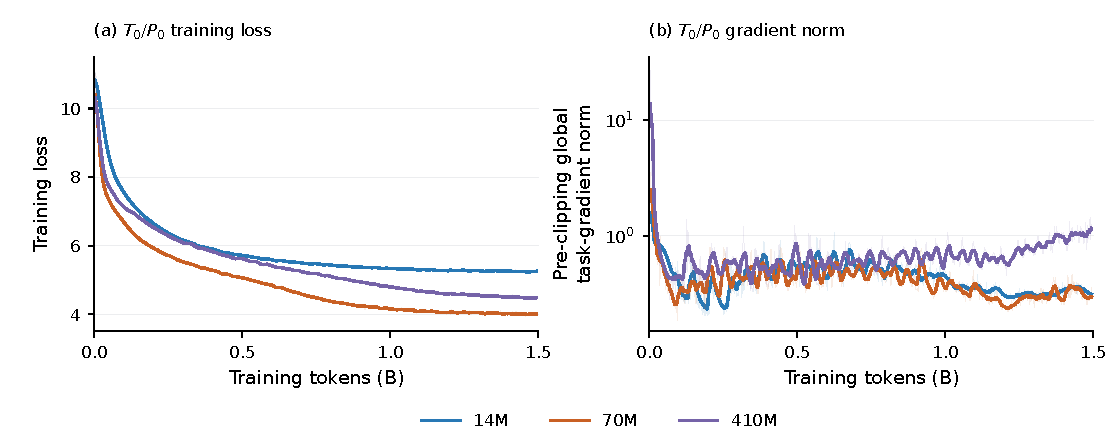
\includegraphics[width=\linewidth]{figures/19-base-model-optimization.pdf}
\caption{\textbf{Base-model ($T_0/P_0$) training at 14M, 31M, 70M and 410M.}
\textbf{(a)} Training loss and \textbf{(b)} gradient norm before clipping
(logarithmic scale). Faint lines show individual updates; solid lines show
centered nine-update means, with shorter windows at the ends. Gradient norms
are computed after accumulation and are not normalized by parameter count.}
\label{fig:a0-optimization}
\end{figure}

\subsection{Training and evaluation}
\label{app:training-protocol}
\label{app:evaluation}

All sizes use the Pythia-14M-deduped tokenizer and seeds of 1234 for
initialization and data order, with one seed per condition. AdamW settings
are shared: $\beta=(0.9,0.95)$, $\epsilon=10^{-8}$, weight decay $0.1$
and gradient clipping at norm $1$. Attention and hidden dropout are zero.
Training uses 712 updates with 1\% linear warmup followed by cosine
learning-rate decay. Table~\ref{tab:training-settings} gives the learning rates,
microbatch sizes and shared effective batch. Gradients accumulate over the
listed microbatches before each optimizer update.
% Scale extension: analyses/038-2026-09-24-base-t2-t7-scale-frontier/observations/003-manuscript-integration.md; 04_manuscript_evidence.py.


The 31M experiment comprises Base and $T_2/P_h$, $T_7/P_h$ at each
$\kappa\in\{0,0.01,0.05,0.1,0.5\}$. Both thresholded recipes use OL1 at $h$
with $\lambda=b=1$. All eleven runs share the same random initial weights,
training-block order, optimizer, learning-rate schedule, token budget and
validation coverage. Base and $T_2/P_h$ come from Run054; $T_7/P_h$ comes
from Run055, with identical initialization and data-order hashes. Training
uses FP16 with dynamic loss scaling and FP32 parameters and optimizer state;
AdamW excludes biases and normalization parameters from weight decay.
These runs extend the threshold-placement comparison with pressure fixed at $h$.

At 14M, the executed conditions include Base, $T_1/P_0$, the $T_1/P_1$
pressure-weight ablation and all seven thresholded recipes in
Table~\ref{tab:interventions}. At 70M, they include Base, $T_1/P_0$,
$T_2/P_h$, and $T_4,T_7$ with $P_h$ or $P_{\mathrm{all}}$;
the additional $T_2/P_h$, $\kappa=0.5$ endpoint was measured in a separate
session. The 410M conditions are Base, $T_1/P_0$ and the five-threshold
$T_4/P_{\mathrm{all}}$, $T_7/P_{\mathrm{all}}$ sweeps.
Validation uses all 500 MiniPile documents: 338 complete 2,048-token blocks
(692,224 input tokens), excluding the final 1,444-token tail. Published
losses use the canonical training evaluation; the BF16 kernel checks below
are a separate numerical qualification.



\FloatBarrier

Figure~\ref{fig:a0-optimization} shows the training trajectories. They do not
establish convergence, and the lower learning rates at 410M limit comparisons
that attribute loss differences to model size alone.
